\section{Auswertung}
Die Auswertung, genauer die Fehlerrechnung, die Plots und Ausgleichsrechnung erfolgt mit den Paketen
Numpy \cite{numpy}, Uncertainties \cite{uncertainties}, Matplotlib \cite{matplotlib} und Scipy \cite{scipy} in der Programmiersprache python.
\subsection{Fehlerrechnung}

\subsection{Kontrastmessung}

\begin{table}[H]
\centering
\begin{tabular}{c|c|c|c}
{$\phi \:/\: \textdegree$} & {$U_\text{max} \:/\: \si{mV}$} & {$U_\text{min} \:/\: \si{mV}$} & {$K$}\\
\midrule
0 & 1394 & 1181 & 0,08 \\
10 & 1194 & 769 & 0,22 \\
20 & 869 & 319 & 0,46 \\
30 & 744 & 175 & 0,62 \\
40 & 781 & 94 & 0,79 \\
50 & 913 & 56 & 0,88 \\
60 & 744 & 90 & 0,78 \\
70 & 919 & 131 & 0,75 \\
80 & 1147 & 469 & 0,42 \\
90 & 963 & 650 & 0,19 \\
110 & 2250 & 344 & 0,74 \\
130 & 1250 & 237 & 0,68 \\
150 & 2156 & 375 & 0,70 \\
170 & 1594 & 813 & 0,32 \\
190 & 1013 & 619 & 0,24 \\
210 & 819 & 188 & 0,63 \\
230 & 1125 & 75 & 0,88 \\
250 & 1297 & 187 & 0,75 \\
270 & 1138 & 788 & 0,18 \\
290 & 2172 & 641 & 0,54 \\
310 & 3562 & 125 & 0,93 \\
330 & 1781 & 375 & 0,65 \\
350 & 1750 & 984 & 0,28 \\
\end{tabular}
\caption{Messwerte der Spannungsextrema der Kontrastmessung.}
\label{tab:kontrast}
\end{table}
\begin{figure}[H]
  \centering
  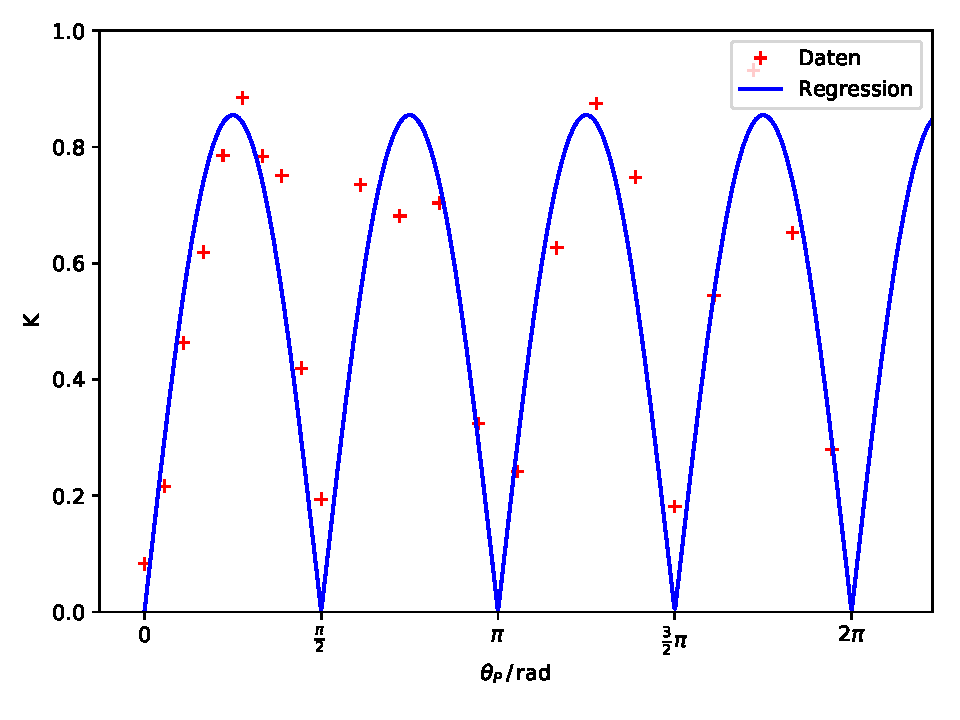
\includegraphics{bilder/kontrastplot.pdf}
  \caption{Kontrast Plot.}
  \label{fig:kontrastplot}
\end{figure}

\subsection{Brechungsindex der Glasplatten}


\subsection{Brechnungsindex von Luft}
